\section{实现进展与待完成工作}

\subsection{目前实现进展}

\subsubsection{数据处理管道（已完成并通过校验）}

已完成从原始数据集到仪表盘数据的\textbf{完整确定性管道}（\texttt{config / normalize / ingest / metrics / qa}），
并对旧版做了地基级重构：

\begin{enumerate}[label=\textbf{\arabic*.}, leftmargin=*, itemsep=0.3em]
    \item \textbf{繁简统一}：OpenCC 繁$\to$简，唐宋词频对比首次干净（不再把繁简差异误当时代差异）。
    \item \textbf{诚实定年}：弃用旧“作者生卒中点分 20 年桶”（被默认年份污染），改为有序时期轴 + 定年阶梯，唐诗可定年 $\approx$ 75\%。
    \item \textbf{范围纠错}：发现宋词语料实为全宋词（含大量南宋），改用词人表 + 生年阈值区分北宋/南宋。
\end{enumerate}

\begin{keybox}[端到端校验（qa.py 全部通过）]
语料 78\,648 首；datable 70\%；\textbf{简体文本繁体残留 = 0}；所有仪表盘 JSON 严格可解析；
时期序列按 盛唐$\to$中唐$\to$晚唐五代$\to$北宋$\to$南宋 单调；去重与定年对账一致。
\end{keybox}

\subsubsection{初步分析发现（核心结果）}

确定性指标已能复现并量化核心叙事，且在 \texttt{full} 与 \texttt{representative} 两个范围下趋势一致（结论稳健）。

\begin{figure}[H]
    \centering
    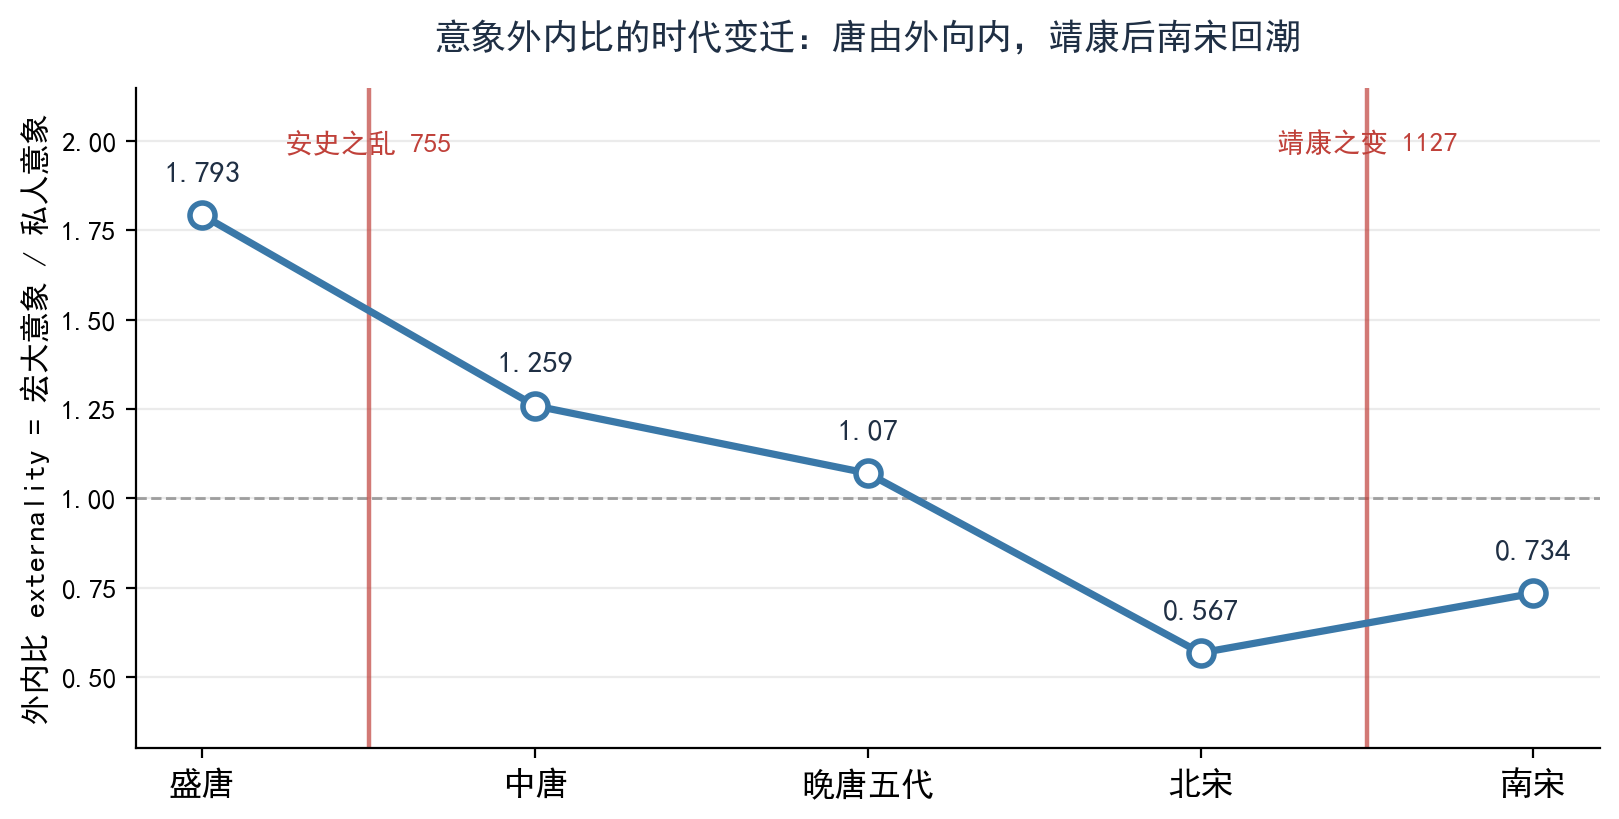
\includegraphics[width=0.92\textwidth]{figures/fig_externality}\\[4pt]
    {\small\heiti 图 1\quad 意象外内比（宏大意象 / 私人意象）的时代变迁}
\end{figure}

\begin{findbox}[关键发现]
外内比：盛唐 1.79 $\to$ 中唐 1.26 $\to$ 晚唐 1.07 $\to$ 北宋 0.57 $\to$ \textbf{南宋 0.73（回升）}。
唐代“由外向内”清晰可见，北宋内向最深；而\textbf{靖康之变后南宋外向性回潮}——
辛弃疾、陆游的家国激愤使“万里/西风”等宏大意象反弹。这一“反弹”是单调“外$\to$内”叙事无法解释的，
正是本项目最有价值的发现。
\end{findbox}

\begin{figure}[H]
    \centering
    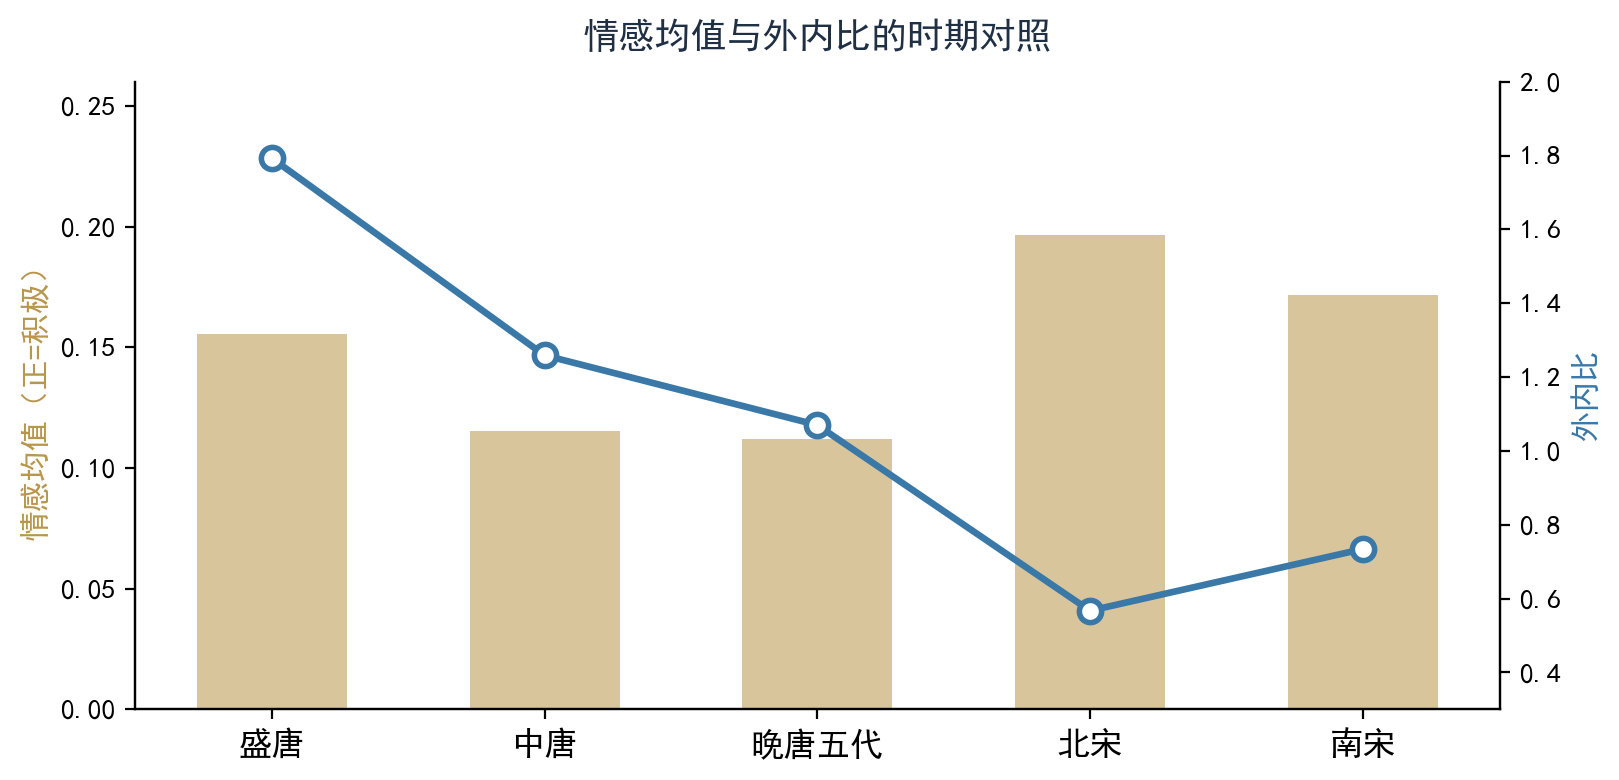
\includegraphics[width=0.92\textwidth]{figures/fig_sentiment}\\[4pt]
    {\small\heiti 图 2\quad 情感均值与外内比的时期对照}
\end{figure}

此外：两大断裂断面已自动产出——靖康断面中南宋升频词含“万里/西风/家国”信号，
策展名篇精准命中辛弃疾《永遇乐·京口北固亭》、陆游、岳飞等；唐宋独有词在繁简统一后呈清晰分野
（唐“心/身/城/门/名”偏外、实，宋“东风/江南/梅花/归去/回首”偏婉约、私人）。

\subsubsection{文档与封面}

项目报告（背景/任务/数据/设计）、数据处理记录、\texttt{pipeline/README} 均已就绪；
本报告主题封面（水墨时间长河 + 繁星 + 两大断裂）为自制。

\subsection{待完成的工作}

\begin{enumerate}[label=\textbf{\arabic*.}, leftmargin=*, itemsep=0.3em]
    \item \textbf{前端仪表盘}：用 React + Vite + ECharts 渲染六屏叙事，落地“流 + 繁星”双层、
          两大断裂断面屏与诗歌地图，并实现多视图联动。
    \item \textbf{案例展示}：待系统跑通后补充真实截图与可复现的交互路径（如下钻杜甫安史名篇、辛弃疾靖康名篇）。
    \item \textbf{细节优化}：词频加停用词表（滤“了/是”等虚词）；宋词三百首匹配率（约 76\%）改首句匹配提升。
    \item \textbf{可选增强}：LDA 主题河流、诗人社交网络（有余力再做）；LLM 作为可选附件做细腻情感类型标注。
    \item \textbf{系统文档与答辩}：期末补齐设计需求/介绍/案例/AI 使用声明，准备 Demo 视频与现场演示。
\end{enumerate}
